%%%%%%%%%%%%%%%%%%%%%%%%%%%%%%
%%%%%%%% Motivation %%%%%%%%%%
%%%%%%%%%%%%%%%%%%%%%%%%%%%%%%
\chapter{Motivation}

Nowadays machine learning and deep learning have become a distinguished approach for visual
recognition tasks and has achieved great success in this process. However, they seek a large amount of
labeled data to learn. Providing this amount of labeled data not only will bring much effort along but also will occupy a huge size of storage and seek large storage. In
contrast, humans are very good in visual recognition so that, they can learn with one \footnote{This
  is known as one-shot learning in deep learning and represents the scenario when there is one
  instance of each class in training-set to learn.} or few \footnote{This is known as few-shot learning in
  deep learning and represents the scenario when there are just few instances of each class in
  training-set to learn.}
examples. Imagine one kid who can recognize a lion in a picture
after looking a few pictures of lions as an example. We want to simulate and apply this human’s
ability to
the deep learning and make them learn with few examples, with desirable accuracy.
In this bachelor thesis, we concern ourselves with few-shot learning in deep learning. We aim to
learn and train a model when there are few labeled examples obtainable. We approach to generate
artificial examples from a few available labeled examples and enalrge our dataset artificially.
This technique known as data augmentation. These artificial labeled examples aid us to learn better
with more accuracy and prevent overfitting. Data augmentation is our focus in this work to achieve few-shot
learning and prevent overfitting. In this thesis, we will introduce different well-known methods of
data augmentation. The first purpose will be to discover if and how far data augmentation can
improve the learning process and accuracy. The second step will be to compare their accuracy. In
the end, we aim to discover the potential possibility of combining the different methods of data
augmentation to increase accuracy and reduce error-rate and improve the learning process.
We will focus on visual recognition tasks and their classification. Additionally, we will concentrate on the implementation of various methods of data augmentation for convolutional neural networks


%%%%%%%%%%%%%%%%%%%%%%%%%%%%%%
%%%%%%%% Introduction %%%%%%%%
%%%%%%%%%%%%%%%%%%%%%%%%%%%%%%
\chapter{Introduction}

Neural networks can possibly contain multiple non-linear layers and this makes them very expressive models
that can learn very complicated relationships between their inputs and outputs. With even limited
input data, neural networks can discover and learn many relations from the data, however, sometimes the
discovered and learned relations do not exist or just consist of redundant information and
relations. Redudant relation can potentially arise of data-noise or lack of data-generalization. Non
exist relations can potentially emerge from lack of enough data. These phenomena known as
\textit{overffiting} in deep learning. In other words, learning with few labeled examples or noisy
data causes overfitting. Overffiting cause low accuracy and high error-rate. Hence, we approach to propagation of artificial
labeled examples from a few given examples to prevent overfitting and reduce the error rate and increase
the accuracy.

As we mentioned aquiring a huge labeled dataset is expensive and seeks much effort and time. Therefore we aim to generate artificial example from few obtainable labeled examples. In other words, we
augment our data and this strategy is known as data augmentation. There are a few well-known methods for data augmentation. We aim to introduce them in this thesis.  Besides we will implement these
methods to compare their efficiency and capability. These methods are as follow:
\begin{itemize}
  \item \textbf{Label Preserving Transformation} \ref{tit:label-preserving}
  \item \textbf{Elastic Distrotion} \ref{tit:elastic-distrotion}
  \item \textbf{Stroke Warping} \ref{tit:stroke-warping}
  \item \textbf{Bayesian Approach} \ref{tit:bayesian-approach}
        %\item \textbf{Manifold Approach} \ref{tit:manifold-approach}
        %\item GANs
\end{itemize}



%%%%%%%%%%%%%%%%%%%%%%%%%%%%%%
%%%%% Data Representation %%%%
%%%%%%%%%%%%%%%%%%%%%%%%%%%%%%
\chapter{Data Representation}
Here should be an Introdution of chapter and introduce the data

\section{MNIST}
The MNIST dataset (Modified National Institute of Standards and Technology) is a large handwritten
digits dataset, provided by Yann Le Cun, derived from NIST Special Database 19 \cite{NIST}.

The MSNIT dataset consists of $60,000$ train- and $10,000$ test-images and each image is grayscale
with $28 \times 28$ pixels. It has $10$ classes that represent $0-9$ digits and data is fairly
splitted between classes \cite{MNIST_data_reference}. MNIST is one of the most popular datasets for
deep learning because of the not too high complexity and compatibility with almost all deep learning
models. Hence many papers attempted to reach a low error-rate on this dataset. One of them manages
to reduce the error-rate on the MNIST by up to $0.23\%$ \cite{MNIST_best_result_reference}. You can
find the information about the dataset at table
\ref{dataset_table} and figure \ref{fig:mnist_dataset_example} shows an example of the dataset.

\begin{figure}
  \centering
  \label{fig:mnist_dataset_example}
  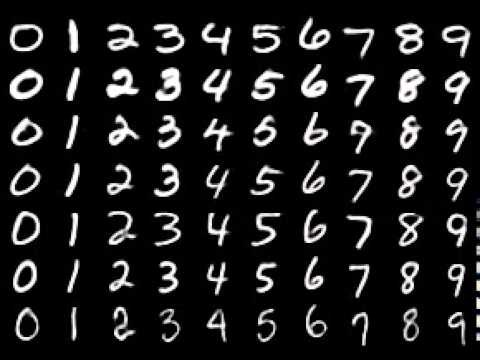
\includegraphics[width=0.5\textwidth]{fig/mnist}
  \caption{7 examples per class of MNIST dataset, merged in one image \cite{MNIST_dataset_example}}
\end{figure}


\section{Fashsion-MNIST}
blablabla


\section{CIFAR-10}
The CIFAR-10 (Canadian Institute for Advanced Research)
, collected by Alex Krizhevsky, Vinod Nair, and Geoffrey Hinton is a subset from 80 million tiny
images dataset \cite{CIFAR-10_origin_dataset}.

The dataset consists of $60,000$  RGB with $32 \times 32$ pixels images, which are divided to the $50,000$ train and $10,000$ test datasets. As the name makes it clear the CIFAR-10 contains 10 classes ([plane, car, bird, cat, deer, dog, frog, horse, ship, truck]) \cite{CIFAR-10_dataset_reference}.
One of the lowest reported error-rate with a convolutional neural network managed to achieve $2.56\%$ \cite{CIFAR-10_best_result_reference}.  You can
find the information about the dataset at table
\ref{dataset_table} and figure \ref{fig:cifar-10_dataset_example} shows an example of the dataset.

\begin{figure}
  \centering
  \label{fig:cifar-10_dataset_example}
  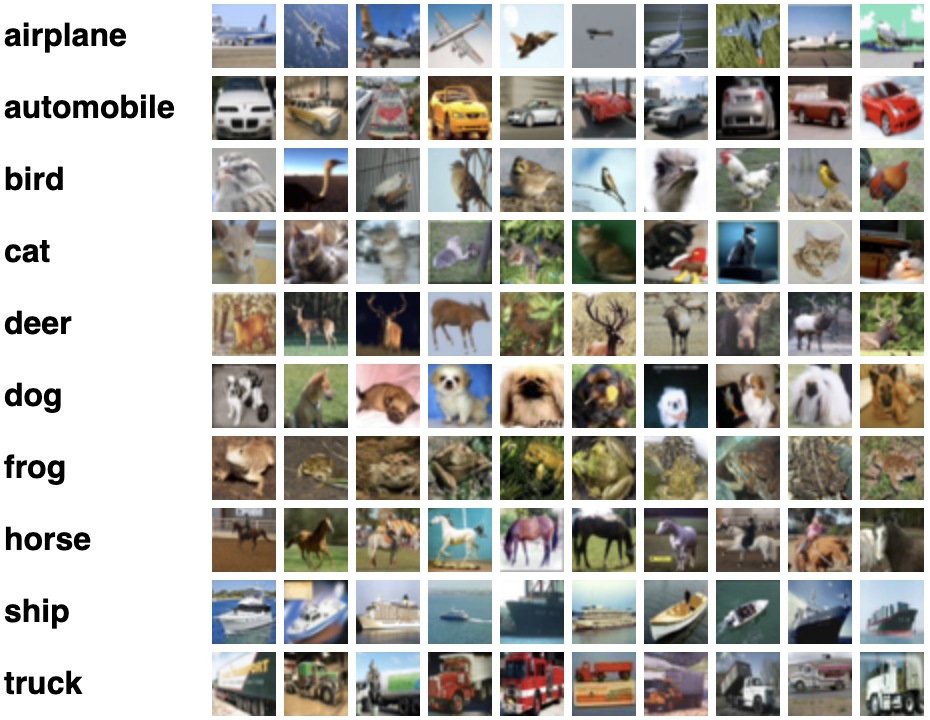
\includegraphics[width=0.5\textwidth]{fig/cifar-10}
  \caption{10 examples per class of CIFAR-10 dataset, merged in one image \cite{CIFAR-10_dataset_reference}}
\end{figure}


\section{CIFAR100}
blablabla


\begin{table}[]
  \label{dataset_table}
  \begin{tabular}{
      l |
      c
      c
      c
      c
      c}
    \hline
    {\textbf{Dataset}}        & \multicolumn{1}{l}{{\textbf{NO. Classes}}} & \multicolumn{1}{l}{{\textbf{NO. Train}}} & \multicolumn{1}{r}{{\textbf{NO. Test}}} & \multicolumn{1}{l}{{\textbf{Size (pixel)}}} & \multicolumn{1}{l}{{\textbf{NO. Channel}}} \\ \hline
    {\textbf{MNIST}}          & 10                                         & 60,000                                   & 10,000                                  & $28\times28$                                & 1 (Grayscale)                              \\
    {\textbf{Fashsion-MNIST}} & 26                                         &                                          &                                         &                                             &                                            \\
    {\textbf{CIFAR-10}}       & 10                                         & 50,000                                   & 10,000                                  & $28\times28$                                & 3 (RGB)                                    \\
    {\textbf{CIFAR100}}       & 100                                        &                                          &                                         &                                             &                                            \\ \hline
  \end{tabular}
  \caption{Structure and organization of the datasets.}
\end{table}


%%%%%%%%%%%%%%%%%%%%%%%%%%%%%%
%%%%% Neural Network %%%%%%%%%
%%%%%%%%%%%%%%%%%%%%%%%%%%%%%%
\chapter{Preliminaries}
\section{Introduction}
\section{Convolutional Neural Network}
\section{Overffiting}


%%%%%%%%%%%%%%%%%%%%%%%%%%%%%%
%%%%%%% Data Augmentaion %%%%%
%%%%%%%%%%%%%%%%%%%%%%%%%%%%%%
\chapter{Data Augmentaion}
Here should be Introdution for data augmenation


\section{Label Preserving Transformation}
\label{tit:label-preserving}

One of the most in common method to enlarge the dataset artificially is the label preserving transformation. This method provides the possibility to generate artificial data with
non-heavy computation. The advantage of a very little computation aids us to save storage. In other
words, it wouldn't be required to save the generated data on a storage and the data can always be
enlarged artificially in a short time and with a little computation. As the method's name makes it
clear, this method aims to generate new data from a single data with the same label. We explain the method and its approach for image datasets because as we mentioned our focus is image datasets.

This method consists of generating image translations and horizontal reflectins. Image translations mean, random patches from the original images. The size of the patches are smaller than the
size of the original images. We will extract all pssobile translations (all possible patches which fit in the image) from our image.
These extracted translations (extracted random patches) and their horizontal reflection will be used
for training our network. Given a single channel (grayscale) n$\times$n image and the translation
pathce with size of m$\times$m and $n>m$ then the training dataset will increase by a factor: $$2\times(n-m+1)\times(n-m+1)$$ In the figur \ref{fig:label-preserving-trasformation} is the process of the translations
and reflections of a small image presented.

At test time, the method extracts the patches with the same size. This time the patches will be extracted from 4 corners and center of the original image. The network predicts on these
five patches and their horizontal reflections (10 patches altogether). In the end, the average
of the predictions will be our network's prediction.

\begin{figure}
  \centering
  \label{fig:label-preserving-trasformation}
  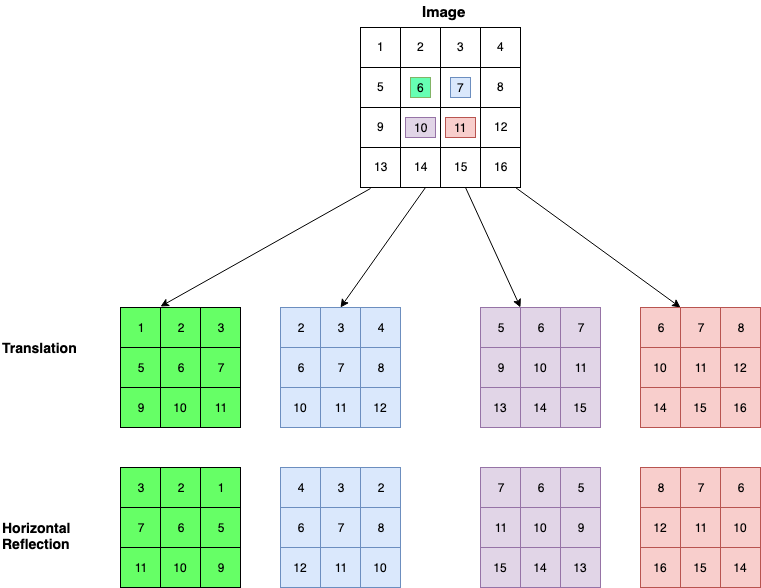
\includegraphics[width=1\textwidth]{fig/label-preserving-transformation}
  \caption{An example of single channel image with size of $4\times4$ with its translations with size of $3\times3$ patches and their horizontal reflections. The numbers determinate the pixels intensity}
\end{figure}


\section{Elastic Distrotion}
\label{tit:elastic-distrotion}
Another well-known method for data augmentation is elastic distortion. This method as the same as label preserving transformation generates artificial data (images) from a single data (image) but with
this difference that this time instead of resizing the image (translation) the pixels inside of the image will be moved and displaced. The intensity of pixels also will be changed with respect to
their new places and their neighbors' intensity and their old places and their origin intensity.

As it cleared elastic distortions concerns itself with a displacement of the pixels and an adjustment of the pixels intensity. This approach is known as interpolation. There are a few schemes like
(nearest neighbor-, bicubic-,  spline- and bilinear interpolation) to reach the goal. Bilinear interpolation is one of the simplest with a desirable result. Hence we use bilinear interpolation. We
will explain the process below.

We will start with pixels displacement. For instance if $\Delta x(x,y)= \alpha x$ and $\Delta y(x,y)= \alpha y$, this means that each pixels will be moved $\alpha x$ in the direction of x-axis and
$\alpha y$ in the direction of y-axis. $\alpha$ would be our scale parameter and since $\alpha$ can be a non-integer value, interpolation is necessary and as we mentioned we use the bilinear
interpolation.  In the next step after pixels displacement, the intensity of the pixels in the new locations should be adjusted concerning the intensity of the neighbors' pixels in the original image
(origin square). Hence bilinear interpolation aids us to reach this target. The bilinear interpolation interpolates the moved pixel horizontally. Then it interpolates the pixel vertically with respect
to yielded values from horizontal interpolations. We will show and summarize the process formally in below.

\begin{definition}{}
  Given $p'$ the pixel which we want to dispalacment it with $\Delta x(x,y)= \alpha x$ and $\Delta y(x,y)= \alpha y$ and $p_{(x,y)}, p_{(x+1,y)}, p_{(x,y-1)}, p_{(x+1,y-1)}$ are the neighbors (on
  origin square) of $p'$ in the new location after displacment and $I(p)$ shows the intensity of pixel $p$. Then the vertical interploation yields:

  $$V_1 = I(p_{(x,y)}) + \big( \Delta x(p', p_{(x,y)}) \times I(p_{(x+1,y)}) \big)$$
  $$V_2 = I(p_{(x,y-1)}) + \big( \Delta x(p', p_{(x,y-1)}) \times I(p_{(x+1,y-1)}) \big)$$

  And then the horizontal interploation yields a new intensity for pixel $p'$ after displacment:
  $$I(p') = V_1 + \big( \Delta y(p', p_{(x,y-1)}) \times V_2) \big)$$
\end{definition}

To reach elastic deformation or elastic distrotion we approach to generate $\Delta x(x,y)= \alpha x$ and $\Delta y(x,y)= \alpha y$ with $\alpha \times rand(-1,+1)$ since $\alpha$ is image-scale parameter
and $rand(-1,+1)$ generate a number between $-1$ and $+1$ with uniform distribution. After all, the
fields $\Delta x$ and $\Delta y$ are convolved with a Gaussian filter with standard deviation of
$\sigma$. The values of $\sigma$ and $\alpha$ depends on the image size and the image entropy. This process will generate elastic deformed image from orginal image which called elastic distrotion.


\section{Stroke Warping}
\label{tit:stroke-warping}
This method as same as previously introduced methods uses predetermined families of transformations.
In other words, we enlarge our dataset artificially with the aid of well-known classical computer
vision transformations. This method notwithstanding of non-heavy complexity accomplished desirable
results even on medical purposes \cite{stroke_tumor}. The ideas of this methode raised from Tangent
Dist \cite{stroke_idea_1992} and Tangent Prop \cite{stroke_idea_1993} works.

In this method, we perform small changes in images to augment our data.  That means we augment our
images with skewing, rotating and shearing (scaling) them \cite{storke_warping_1997_source}. As same as the
label preserving transformation and elastic distortion the augmentation will be started before the
training phase and the training will be performed on enlarged data. Figure
\ref{fig:stroke_warping_transforamtions} represents each mentioned transformation to make them visually
understandable.

\begin{figure}
  \centering
  \label{fig:stroke_warping_transforamtions}
  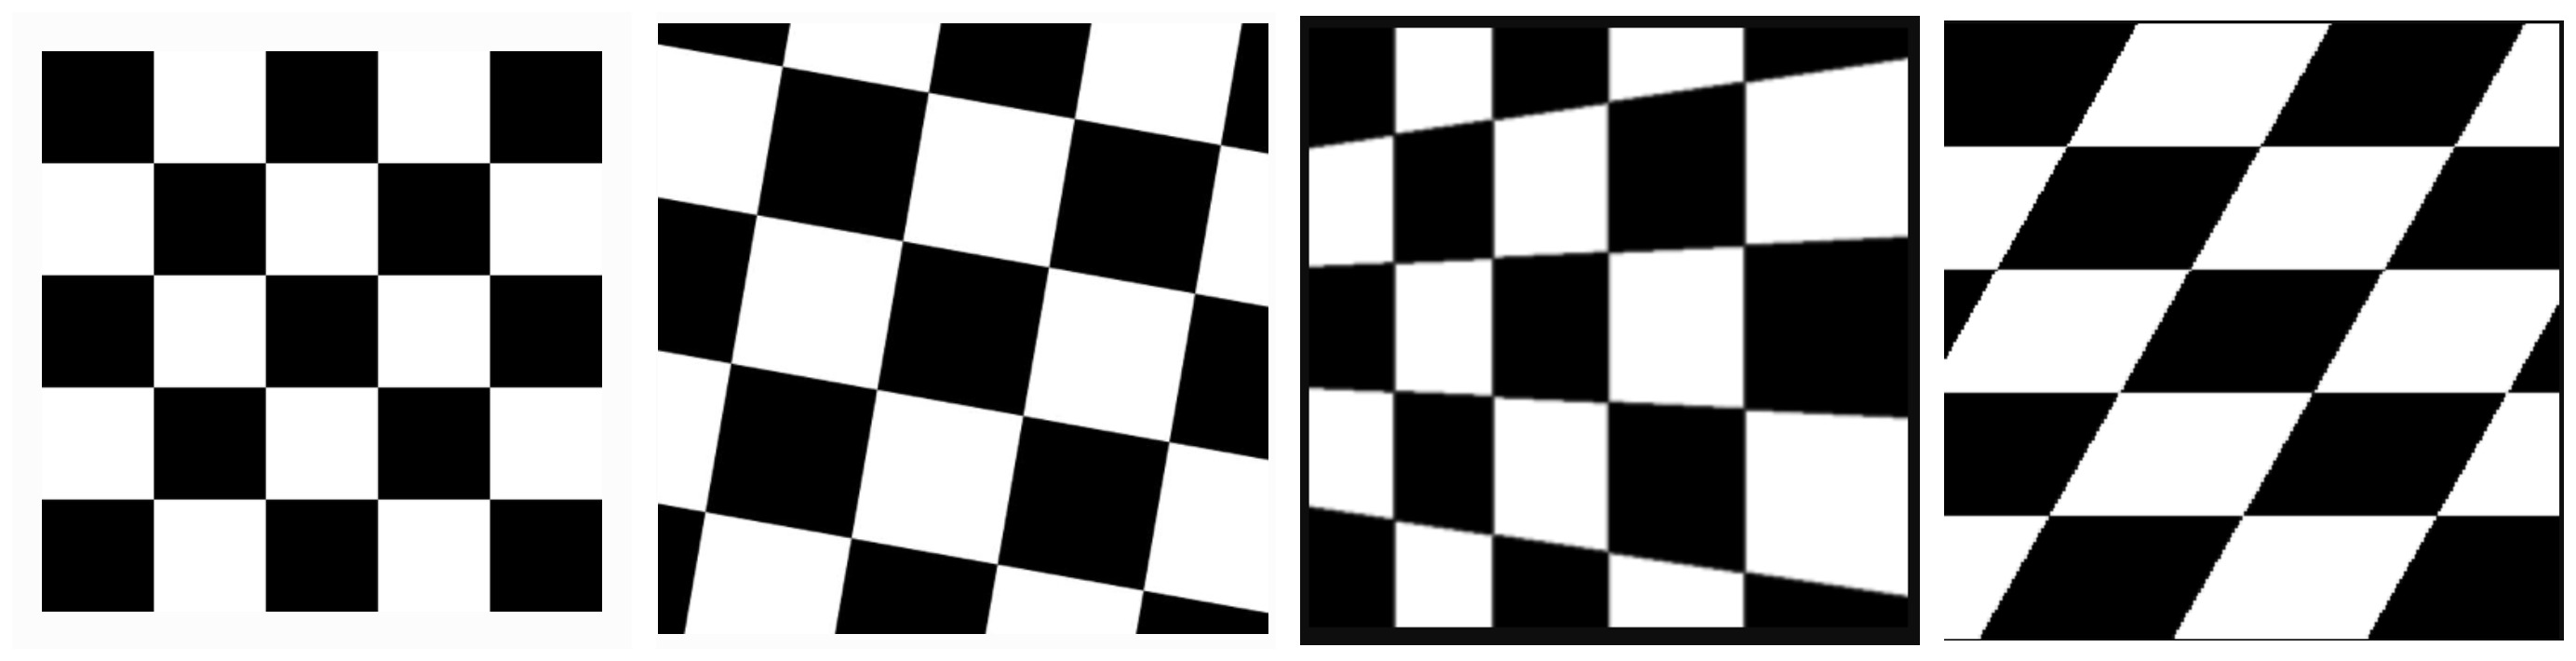
\includegraphics[width=1\textwidth]{fig/stroke_warping_transforamtions}
  \caption{An exmaple of rotation, skew, and shear (scale) transforamtions for stroke warping respectively from left to right \cite{TODO-Augmentaion}}
\end{figure}


\section{Bayesian Approach}
\label{tit:bayesian-approach}
As you may until now realized, all introduced classes of techniques in this work for data
augmentation were pre-defined families of statistical transformations. In other words, we generated
synthetic images with computer vision techniques statistically before the training phase and our
augmented data generated once and during the learning process we didn't change them. In fact, the basic idea of each of
them is known as “poor man’s” data augmentation (PMDA) \cite{poor_man_data_augmentation}. The point
is if neural networks, in general, can learn such complex relations and patterns in images,
therefore they should be able to learn latent variables to improve data augmentation dynamically.
Put the matter another way, in this method, we focus not only on the classification task and
learning patterns of images but also on learning how to improve our image augmentation dynamically
and iteratively during the training and classification.

Before we start with the description of the Bayesian approach, it would be necessary to introduce
generative models or more especially Generative Adversarial Networks (GANs). One of the remarkable
works on GANs proposed by Goodfellow et al. \cite{TODO}. In the below first, we
will introduce GANs and after that and in the Bayesian approach description we will explain how this
approach uses the main idea of GANs and extend it to improve data augmentation.

\subsection{Generative Adversarial Network (GAN)}
\label{tit:Generative-Adversarial-Network}
A Generative Adversarial Network (GAN), in general, consists of two parts:
\begin{itemize}
  \item \textbf{Generator}: As the name cleared itself, it tries to generate new data and simultaneously learns how to generate the data more plausible.
  \item \textbf{Discriminator}: The discriminator learns to distinguish generated fake data from the generator and real data. Besides, it helps and teaches the generator like a kind teacher to generate more plausible data and close to real.
\end{itemize}

Indeed the generator and the discriminator play a minimax game. In other words, the generator
tries to fool the discriminator with fake data and the discriminator tries to distinguish this
matter and tell the generator that he failed to fool and helps the generator to generate data
closer to real ones. In the beginning, the discriminator can simply distinguish the real data and
the generator's fake data. But after each iteration, the generator becomes more intelligent and
generates more plausible data.  In the end, the generator becomes so intelligent so that it can
almost fool the discriminator. This means, that the discriminator's accuracy reduces to about
$50\%$. In effect, the discriminator predicts almost randomly while it predicts between $2$ labels
(real or fake). Sometimes it is even hard for humans to distinguish the
generator's fake data and real data.

The generator will be fed by random\footnote{noise}
input to generate synthetic data. In general, GANs try to replicate a probability distribution. For this matter, they use loss function to measure the distance between the distribution of the generator's data and the distribution of the real data. As we mentioned Goodfellow el al. \cite{Same} suggest minimax loss in their work. The minimax loss defined as:

\begin{equation} \label{eq:minimax_loss}
  Minimax\ Loss = E_{x}[\log (D(x))]+E_{z}[\log (1-D(G(z)))]
\end{equation}


where $D(x)$  denotes the discriminator's estimate of the probability that real data instance x is
real and $D(G(z))$ denotes the discriminator's estimate of the probability that a fake instance is
real. It is clear that the Generator tries to minimize the (\ref{eq:minimax_loss}) and the
discriminator tries to maximize it. Figure \ref{fig:gan_architecture} shows a basic architecture of a
GAN.

\begin{figure}
  \centering
  \label{fig:gan_architecture}
  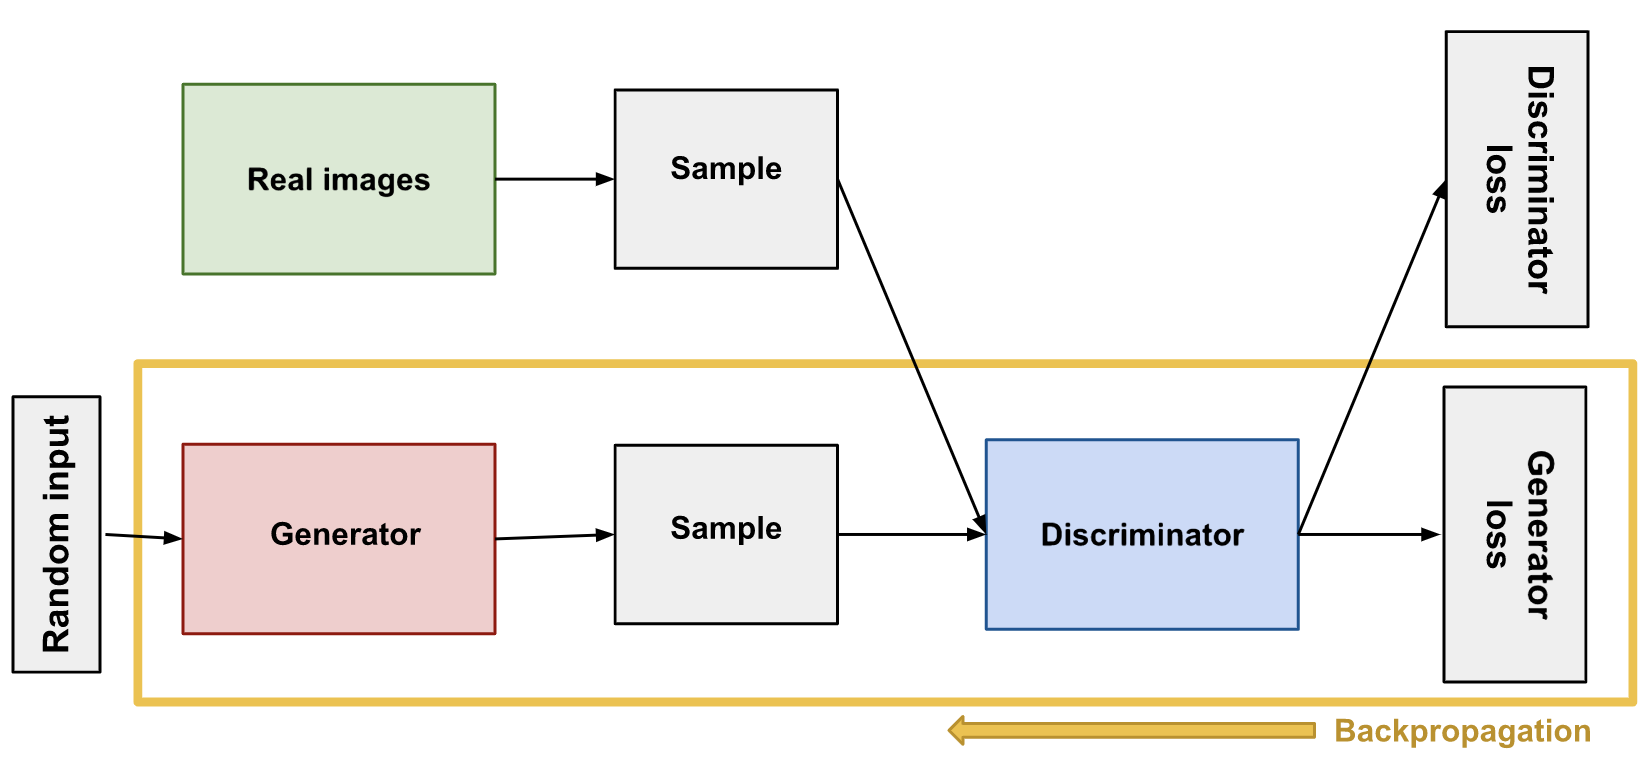
\includegraphics[width=1\textwidth]{fig/gan_architectur}
  \caption{GAN architecture
    \cite{TODO-google-reference}}
\end{figure}

Now and after briefly introduction of GANs we can start with the \textbf{Bayesian Approach}. One of
the noteworthy work for data augmentation with the aid of the bayesian model proposed by Toan Tran
et al. \cite{bayesian_approach}. In this approach, our deep learning model tries to estimate the
distributions of labeled data and with aid of the estimated distributions optimizes the latent
variable used for data augmentation. The approach uses the GANs architecture skeleton to generate
synthetic data with the difference that the optimization of latent derived from the Bayesian model.
The principle idea for data augmentation using latent variables proposed by the statistical learning
community \cite{Statistical_data_augmentation}. Nevertheless applying the idea, directly into deep
learning seeks a massive computational effort. Therefore we talked before about the estimation. To
be more precise, the
approach uses a novel Bayesian data augmenation algorithm, called Generalized Monte Carlo Expectation Maximization
(GMCEM). This algorithm augments training data and mutually optimizes the network parameters. The
algorithm successively generates synthetic data and use Monte Carlo to estimate the expected value
of the network parameters given the previous estimate instead of calculating loss function. After
the estimation of the expected value, the parameter values will be updated with stochastic gradient
descent (SGD). In the end, the algorithm and approach turned in to reality with the aid of GANs. The
proposed GAN consists of one generator and $2$ discriminators. As we in the GANs section
(\ref{tit:Generative-Adversarial-Network}) discussed the generator is responsible to generate
synthetic data and one of our discriminators distinguishes fake and real data. However, the second
discriminator discriminates between the classes of data. Figure
\ref{fig:bayesian-approach-gan-architecture} represents the utilized netwok architecture in this
approach visually. This proposed architecture is nearly similar to the Auxiliary classifier GANs
(AC-GANs) \cite{AC-GANS}. Nevertheless, in the AC-GANs discriminator responsible for both
classification real-or-fake data and data labels (classes) and in our network we utilized $2$
discriminators separately for this matter.

\begin{figure}
  \centering
  \label{fig:bayesian-approach-gan-architecture}
  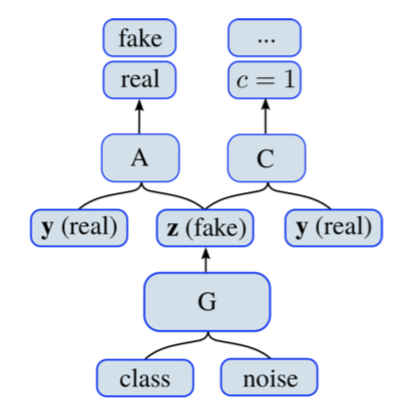
\includegraphics[width=0.5\textwidth]{fig/bayesian-approach-gan-architecture}
  \caption{The network architecture of Bayesian data augmentaion approch \cite{bayesian_approach}. G: Generator, A: Authenticator, C: Classifier.}
\end{figure}

In the following, we will explain the utilized algorithm formally from the Toan Tran el al. work \cite{bayesian_approach}. As we mentioned the goal is to estimate the parameters of the neural networks using labeled data. The training process is defined by the following optimization problem:

\begin{equation} \label{eq:optimization-problem}
  \theta^{*}=\arg \max \log p(\theta | \mathbf{y})
\end{equation}
Where training set denoted as $\mathcal{Y}=\left\{\mathbf{y}_{n}\right\}_{n=1}^{N}$ with $y=(t,x)$
and $t\in\{1, ..., K\}$ (Classes-Set) and data samples $\mathbb{R}^D$ and $\theta$ denoted as
model (network) parameters and observed posterior defined as:
\begin{equation} \label{eq:observed-posterior}
  p(\theta | \mathbf{y})=p(\theta | t, \mathbf{x}) \propto p(t | \mathbf{x}, \theta) p(\mathbf{x} | \theta) p(\theta)
\end{equation}
Now if we assume that the data samples $\mathcal{Y}$ are conditionaly independent, we can define the
following loss function which maximize the (\ref{eq:optimization-problem}).

\begin{equation} \label{eq:loss-function}
  \log p(\theta | \mathbf{y}) \approx \log p(\theta)+\frac{1}{N} \sum_{l}^{N}\left(\log p\left(t_{n} | \mathbf{x}_{n}, \theta\right)+\log p\left(\mathbf{x}_{n} | \theta\right)\right)
\end{equation}
where $p(\theta)$ denotes a prior on the distribution of the deep learning model parameters, $p(t_n|x_n, \theta)$
represents the conditional likelihood of label $t_n$, and $p(x_n|\theta)$ is the likelihood of the
data $x$.

After estimation and optimization the $\theta$ on our training set, it is the time to generate
synthetic data from $y$ using latent variable $z$. Therefore the augmented $p(\theta | y,z)$ can be
estimated. The latent variable $z$ as same as $y$ defined as $z = (t^{\alpha}, x^{\alpha})$ where
$t^{\alpha} \in \{1,...,K\}$ denotes associated label and $x^{\alpha} \in   \mathbb{R}^D$ is
synthesized sample. As we mentioned to avoid a heavy and most likely interminable computation,
instead of the Expectation-Maximization (EM) algorithm we will use Generalized Monte Carlo EM
Algorithm to estimate the expected value and maximize it.Hence the augmented posterior $p(\theta|y,
  z)$ for latent variable $z$ will be as follow:

\begin{equation} \label{eq:latent-variable}
  p(\theta | \mathbf{y}, \mathbf{z})=\frac{p(\mathbf{y}, \mathbf{z}, \theta)}{p(\mathbf{y}, \mathbf{z})}=\frac{p(\mathbf{z} | \mathbf{y}, \theta) p(\theta | \mathbf{y}) p(\mathbf{y})}{p(\mathbf{z} | \mathbf{y}) p(\mathbf{y})}=\frac{p(\mathbf{z} | \mathbf{y}, \theta) p(\theta | \mathbf{y})}{p(\mathbf{z} | \mathbf{y})}
\end{equation}
where the expectation step will be defined as follow:
\begin{equation} \label{eq:expectation-latent-variable}
  p(\theta | \mathbf{y}, \mathbf{z})=\frac{p(\mathbf{y}, \mathbf{z}, \theta)}{p(\mathbf{y}, \mathbf{z})}=\frac{p(\mathbf{z} | \mathbf{y}, \theta) p(\theta | \mathbf{y}) p(\mathbf{y})}{p(\mathbf{z} | \mathbf{y}) p(\mathbf{y})}=\frac{p(\mathbf{z} | \mathbf{y}, \theta) p(\theta | \mathbf{y})}{p(\mathbf{z} | \mathbf{y})}
\end{equation}
where \(\mathbf{z}_{m} \sim p\left(\mathbf{z} | \mathbf{y}, \theta^{i}\right),\) for \(m \in\{1,
\ldots, M\} .\) In \((6),\) if the label \(t_{m}^{a}\) of the \(m^{t h}\) synthesized sample
\(\mathbf{z}_{\mathbf{m}}\) is known, then \(\mathbf{x}_{m}^{a}\) can be sampled from the
distribution \(p\left(\mathbf{x}_{m}^{a} | \theta, \mathbf{y}, t_{m}^{a}\right) .\) Hence, the
conditional distribution \(p(\mathbf{z} | \mathbf{y}, \theta)\) can be decomposed as:

\begin{equation}
  p(\mathbf{z} | \mathbf{y}, \theta)=p\left(t^{a}, \mathbf{x}^{a} | \mathbf{y}, \theta\right)=p\left(t^{a} | \mathbf{x}^{a}, \mathbf{y}, \theta\right) p\left(\mathbf{x}^{a} | \mathbf{y}, \theta\right)
\end{equation}
where \(\left(t^{a}, \mathbf{x}^{a}\right)\) are conditionally independent of y given that all the
information from the training set y is summarized in \(\theta\) this means that \(p\left(t^{a} |
\mathbf{x}^{a}, \mathbf{y}, \theta\right)=p\left(t^{a} | \mathbf{x}^{a}, \theta\right),\) and
\(p\left(\mathbf{x}^{a} | \mathbf{y}, \theta\right)=p\left(\mathbf{x}^{a} | \theta\right)\).
Now with respect to the $\theta$ for the maximization step with concern of removing the independent terms
for $\theta$ will derived the maximization of $\hat{Q}\left(\theta, \theta^{i}\right)$ as follow:

\begin{equation}
  \begin{aligned}
     & \hat{Q}\left(\theta, \theta^{i}\right)=\log p(\theta)+\frac{1}{N} \sum_{n=1}^{N}\left(\log p\left(t_{n} | \mathbf{x}_{n}, \theta\right)+\log p\left(\mathbf{x}_{n} | \theta\right)\right)+\frac{1}{M} \sum_{m=1}^{m} \log p\left(\mathbf{z}_{m} | \mathbf{y}, \theta\right) \\
     & =                                                                                                                                                                                                                                                                           \\
     & \log p(\theta)+\frac{1}{N} \sum_{n=1}^{N}\left(\log p\left(t_{n} | \mathbf{x}_{n}, \theta\right)+\log p\left(\mathbf{x}_{n} | \theta\right)\right)+\frac{1}{M}
    \sum_{m=1}^{n}\left(\log p\left(t_{m}^{a} | \mathbf{x}_{m}^{a}, \theta\right)+\log p\left(\mathbf{x}_{m}^{a} | \theta\right)\right)
  \end{aligned}
\end{equation}

After all, we estimate the $\theta^{i +1}$ so that $\hat{Q}(\theta^{i +1}, \theta^{i}) >
\hat{Q}(\theta^{i}, \theta^{i})$. To reduce the computation complexity as we mentioned instead of
gradient descent, stochastic gradient decent (SGD) utilized for estimating the $\theta^{i +1}$. The
iteration will be continued until $|\theta^{i +1} - \theta^{i}|$ get sufficiently small. 

As we made it clear the above formal explanations and equations are derived from \cite{bayesian_approach} and in some points are matched one-to-one.  

%\section{Manifold Approach}
%\label{tit:manifold-approach}

\chapter{Expriments \& Results}
\section{CNNs Architecture}

\subsection{MNIST}
\subsection{Fashsion-MNIST}
\subsection{CIFAR-10}


\section{Implementaions}

\subsection{Label Preserving Transformations}
\subsection{Elastic Distortion}
\subsection{Stroke Warping}
\subsection{Bayesian Approach}

\section{Results}



\chapter{Comprehensive Comparison}

\chapter{Contribution Of Work}